\documentclass{beamer}

\usepackage[T1]{fontenc}
\usepackage[utf8]{inputenc}
\usepackage{lmodern}
\usepackage{graphicx}
\usepackage[absolute,overlay]{textpos}
\usepackage{multicol}
\usepackage{listings}
\usepackage{svg}

%% Beamer customization--------------------------------------------------------

\usepackage{xcolor}


\usepackage{tikz}

\usetheme{Warsaw}

%% Themes
% Outer themes
\useoutertheme{shadow}
% Rounded boxes and shadows
\useinnertheme[shadow=true]{rounded}
% Solid \item symbols
\useinnertheme{circles}

%% Custom colors
\definecolor{rltgreen}{rgb}{0,0.5,0}
\definecolor{pasteur}{RGB}{0,90,154}
\setbeamerfont{block title}{size={}}
\setbeamercolor{structure}{fg=pasteur}
\setbeamercolor{item}{fg=pasteur}


%Color of title
\setbeamertemplate{frametitle}
{    \nointerlineskip
    \begin{beamercolorbox}[sep=0.3cm,ht=1.8em,wd=\paperwidth]{frametitle}
        \vbox{}\vskip-2ex%
        \strut\insertframetitle\strut
        \vskip-0.8ex%
    \end{beamercolorbox}
}
% Hide navigation symbols
\setbeamertemplate{navigation symbols}{}

%% Title block
\setbeamercolor*{title}{use=structure,fg=white,bg=pasteur}

\makeatletter

%% Top infolines
\setbeamertemplate{headline}{%
\leavevmode%
  \hbox{%
    \begin{beamercolorbox}[wd=\paperwidth,ht=2.5ex,dp=1.125ex]{palette quaternary}%
    \insertsectionnavigationhorizontal{\paperwidth}{}{\hskip0pt plus1filll}
    \end{beamercolorbox}%
  }
}


%% Define Snakemake -----------------------------------------------------------

\definecolor{eclipseBlue}{RGB}{42,0.0,255}
\definecolor{eclipseGreen}{RGB}{63,127,95}
\definecolor{eclipsePurple}{RGB}{127,0,85}

\lstset{language=Python}
\lstset{
    basicstyle=\scriptsize\ttfamily,
    morekeywords={rule, output, shell, params, run, configfile, temp, log},
    showstringspaces=false,
    commentstyle=\color{eclipseGreen}, % style of comments
    keywordstyle=\color{eclipsePurple}, % style of keywords
    stringstyle=\color{eclipseBlue}, % style of strings
}



%% Set up title ---------------------------------------------------------------

\title[Sequana]{Sequana: a set of flexible genomic pipelines for processing 
and reporting NGS analysis}
\author[T. Cokelaer]{Thomas Cokelaer - Dimitri Desvillechabrol}
\institute{Institut Pasteur}
\date{Nov 9th 2017, Paris (séminaire bioinfo Toulouse)}


\AtBeginSection[]{
  \begin{frame}
  \vfill
  \centering
  \begin{beamercolorbox}[sep=8pt,center,shadow=true,rounded=true]{title}
    \usebeamerfont{title}\insertsectionhead\par%
  \end{beamercolorbox}
  \vfill
  \end{frame}
}

\begin{document}

%% Title slide ----------------------------------------------------------------

\begin{frame}[plain]
    \titlepage
    \begin{textblock*}{5cm}(4.5cm,0.3cm)
        
\includegraphics[scale=0.09]{images/Institut_Pasteur.png}
    \end{textblock*}
\end{frame}

%% Slides ---------------------------------------------------------------------




\begin{frame}
\frametitle{Motivation}
\begin{block}{Jan 2015: provide NGS pipelines to Biomics sequencing platform 
https://research.pasteur.fr/en/team/biomics/ (Institut Pasteur)}
 \begin{itemize}
  \item Genomics: QC + variant calling + de-novo
  \item Transcriptomics: RNA-seq + ChIP-seq 
  \item Metagenomics
  \item Illumina but also Pacbio long reads technologies
 \end{itemize}
 %\includegraphics{images/genetic_strand.png}
 %\includegraphics{images/strand.png}
\end{block} 
\end{frame}



\begin{frame}
\frametitle{How ?}

\begin{columns}
\begin{column}{1.5cm}

\includegraphics[height=0.2\textheight]{images/logo_python.png} 
\end{column}
\begin{column}{9cm}
a glue language, a scientific language
\end{column}
\end{columns}


\rule{\textwidth}{1pt}


\begin{columns}
\begin{column}{1.5cm}

\includegraphics[height=0.2\textheight]{images/logo_snakemake.png}
\end{column}
\begin{column}{9cm}
a pipeline 
framework mixing Python and Makefile \\
{\footnotesize \textcolor{blue}{\textit{Köster, Johannes and Rahmann, Sven. 
Snakemake - A scalable 
bioinformatics workflow engine. Bioinformatics 2012.}}}
\end{column}
\end{columns}

\rule{\textwidth}{1pt}


\begin{columns}
\begin{column}{1.5cm}

\includegraphics[height=0.2\textheight]{images/exe.png}
\end{column}
\begin{column}{9cm}
Dedicated standalone such as genome coverage characterisation or a graphical 
user interface for Snakemake pipelines (Sequanix).
%{\footnotesize \textcolor{blue}{\textit{D. Desvillechabrol, C. 
%Bouchier, S. Kennedy, T. Cokelaer Detection and characterization of low 
%and high genome coverage regions .... BioRxiv 
%https://doi.org/10.1101/092478 }}. Submitted to GigaScience journal }
\end{column}
\end{columns}



\end{frame}



\section{Snakemake as a workflow manager}


\begin{frame}
\centering

$\begin{array}{l}

\includegraphics[height=0.18\textheight]{images/logo_snakemake.png}
\end{array}$
{\Huge =}
Makefile 
{\LARGE + }
$\begin{array}{l}

\includegraphics[height=0.18\textheight]{images/logo_python.png}
\end{array}$

See dedicated slides for a Snakemake overview and tutorial on
github.com/sequana/sequana\_presentations
 
\end{frame}



\begin{frame}[fragile]
\begin{block}{configuration file example in YAML format}
 \begin{lstlisting}
##########################################################
# Input parameters for the fractal analysis
#
# :Parameters: 
#
# - size: output image size formatted as NxM where N and M 
#         are integers
# - depth: a integer (e.g. 200)
# - zoom: a positive value e.g. 0.5
# - N: number of random sets
gc:
    - window: 100
    - directory: /home/user/fastq_files
 \end{lstlisting}
\end{block}
\end{frame}



\section{Sequana pipelines (an overview)}


\begin{frame}
\frametitle{Pipeline example: quality control pipeline} 
\centering
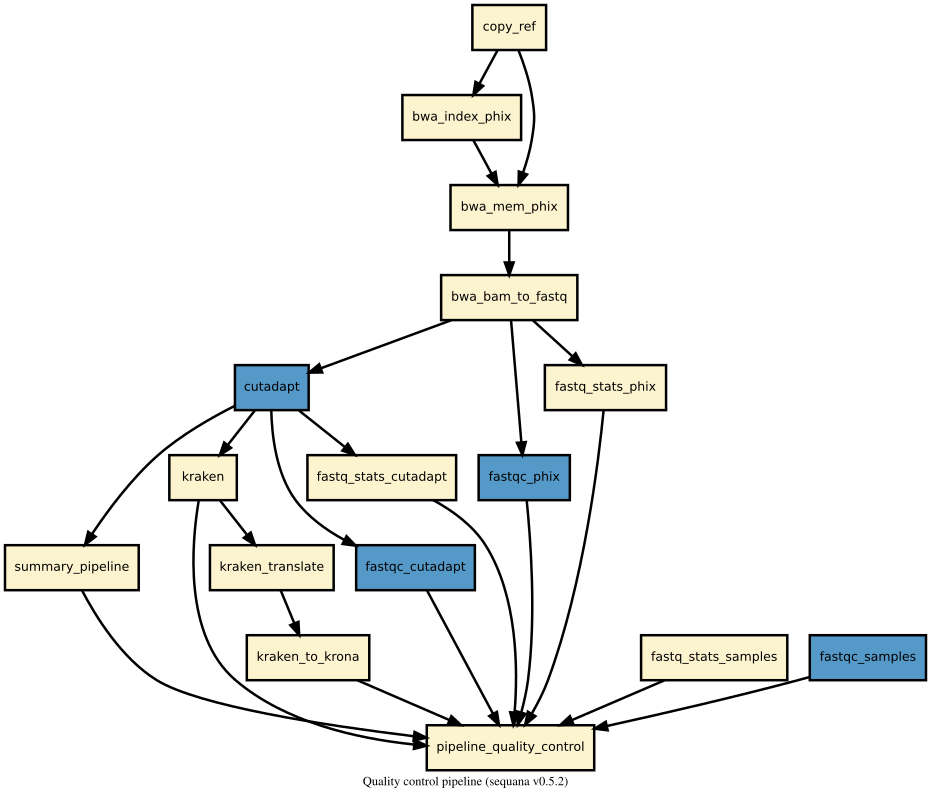
\includegraphics[height=0.8\textheight, width=\textwidth]{./images/dag.png}
\end{frame}



\begin{frame}
\frametitle{Pipeline example: variant calling} 
\centering
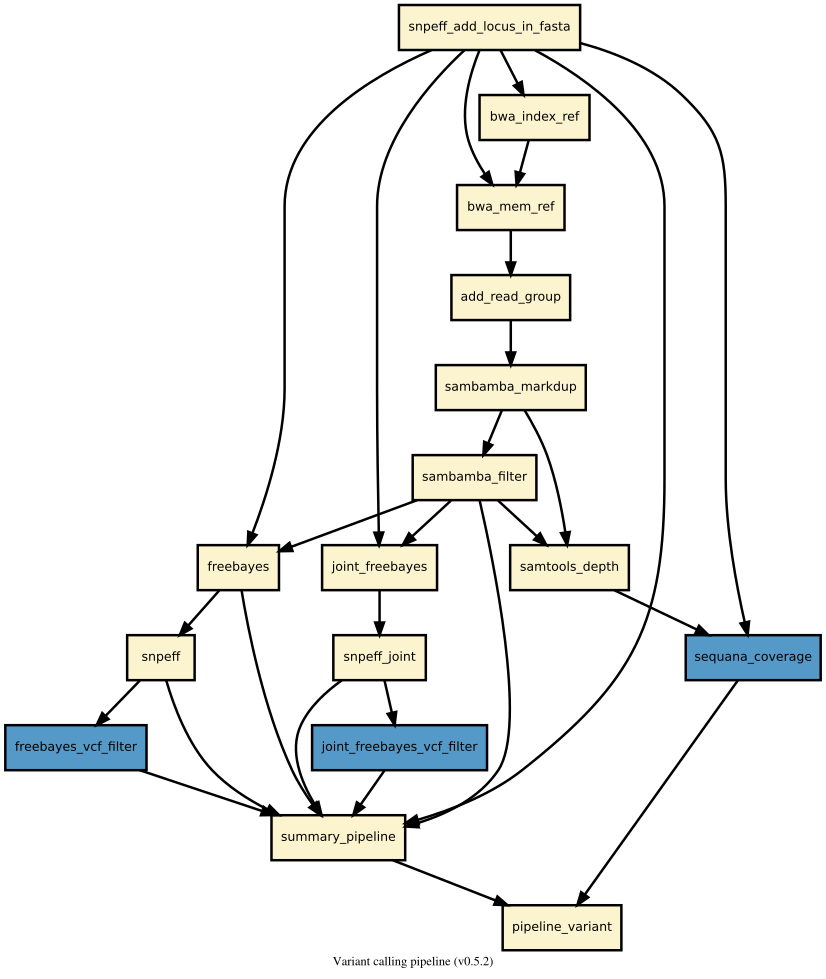
\includegraphics[height=0.8\textheight, 
width=\textwidth]{./images/variant_calling_dag.png}
\end{frame}



\begin{frame}{Pipeline complexity}

    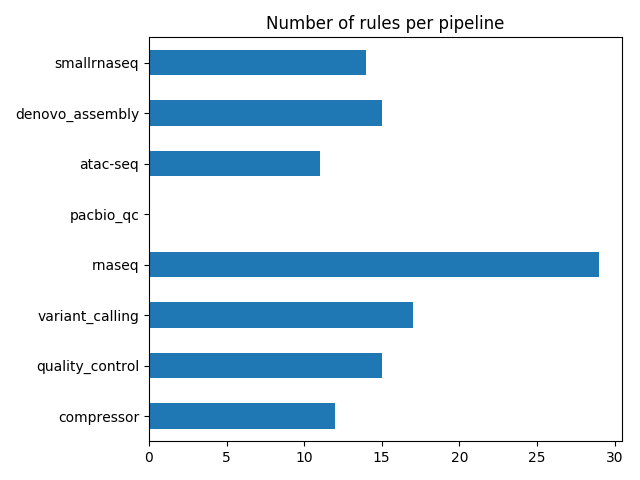
\includegraphics[width=11cm, height=7cm]{images/number_of_rules.png}

\end{frame}


\begin{frame}[fragile]
 \frametitle{Modularization: Factorise and reuse rules}

 
 Local standard rules
\begin{lstlisting}[basicstyle=\ttfamily\small] 
    include: "path_to_rule_file"
\end{lstlisting}

Sequana rules
\begin{lstlisting}[basicstyle=\ttfamily\small]
    from sequana import snaketools as sm
    include: sm.modules['rulegraph']
\end{lstlisting}

Dynamic rules:
\begin{lstlisting}[basicstyle=\ttfamily\small]
    sm.init("quality_control.rules", globals())
    with open(sequana.modules["fastqc_dynamic"], "r") as dynrule:
        exec(dynrule.read())
        
    manager = sm.PipelineManager("quality_control", 
                                 config)

    include: fastqc_dynamic("example1", manager)
    include: fastqc_dynamic("example2", manager)
\end{lstlisting}
\end{frame}


\begin{frame}{Factorization}
\centering
    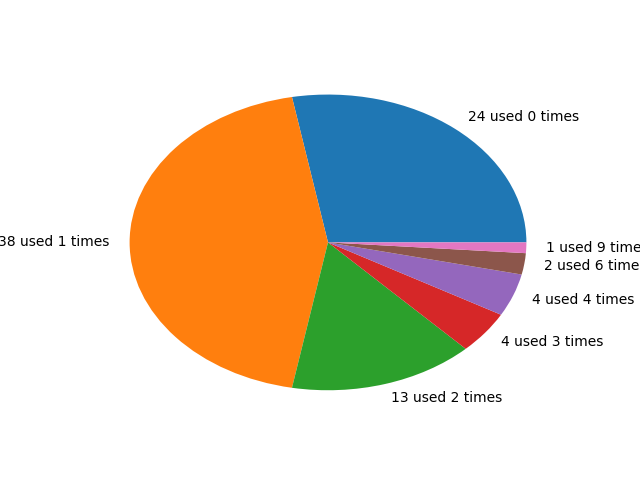
\includegraphics[width=8cm]{images/rules_reusing.png}
\end{frame}


\begin{frame}
 
Once upon time there was a pipeline ... and a configuration file.

\vspace{1cm}
\pause


One need to edit the configuration file ... without typos 
 
 \vspace{1cm}
\pause

One need to launch the Snakemake command ... without typos
 
\end{frame}


\section{Sequanix}
\begin{frame}{GUI to simplify the usage of snakemake}
    \begin{columns}
        \begin{column}{0.5\textwidth}

            \only<1>{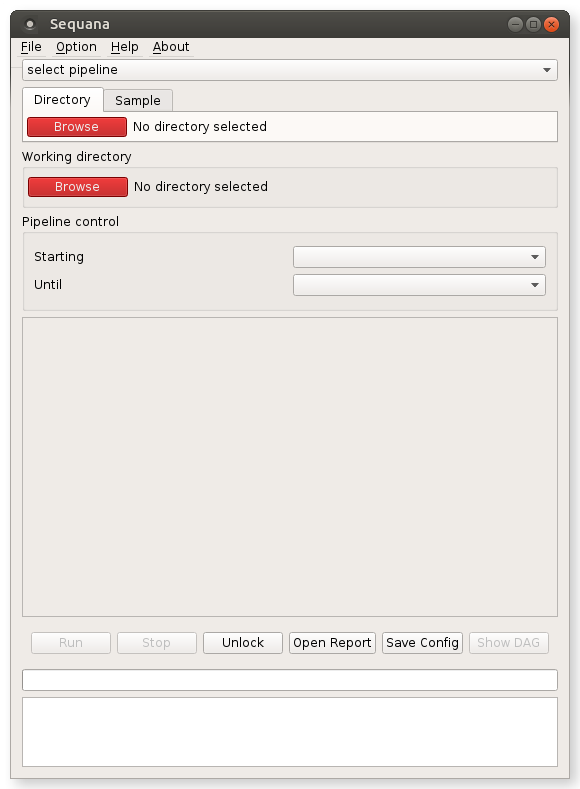
\includegraphics[scale=0.25]{../../images/sequana_init}}

            \only<2>{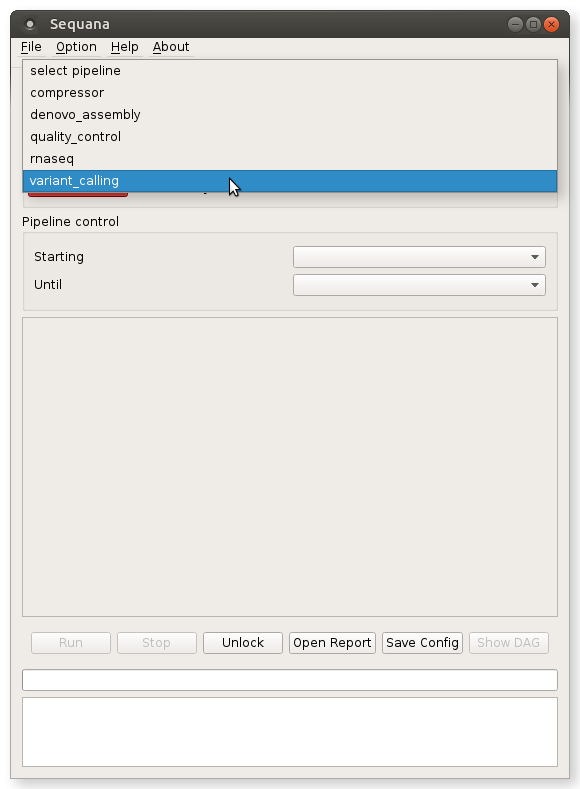
\includegraphics[scale=0.25]{../../images/choose_pipeline}}

            \only<3>{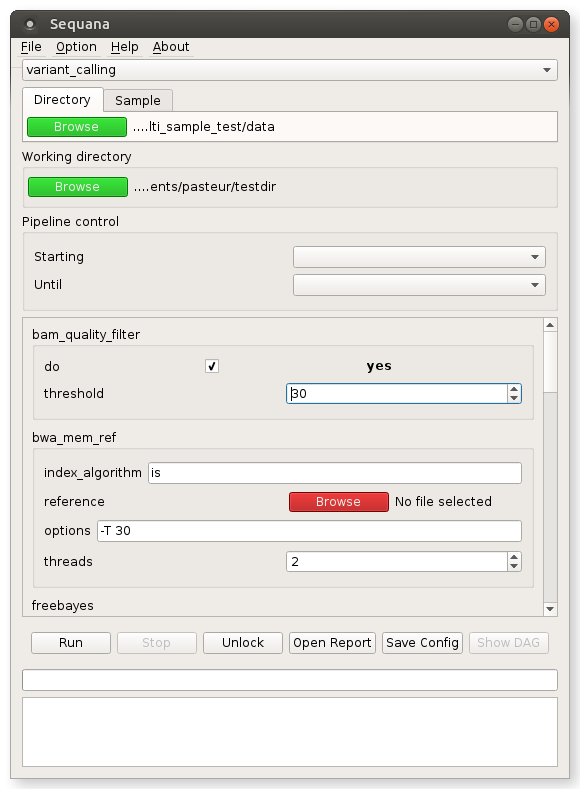
\includegraphics[scale=0.25]{../../images/choose_input_output}}

            \only<4>{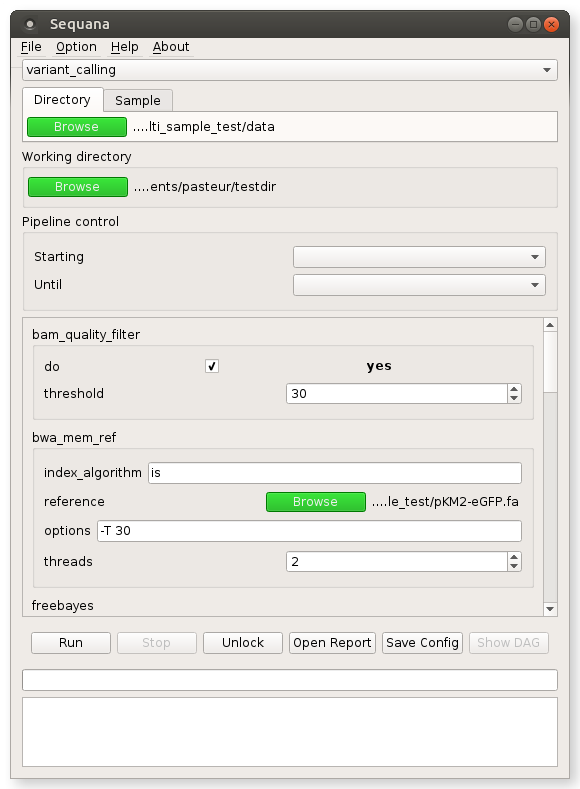
\includegraphics[scale=0.25]{../../images/sequana_pipeline}}

            \only<5>{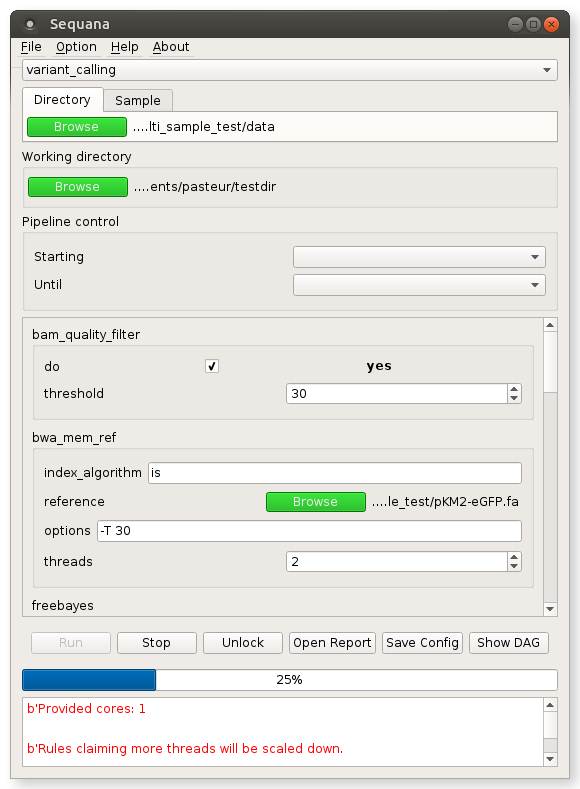
\includegraphics[scale=0.25]{../../images/sequana_running}}

            \only<6>{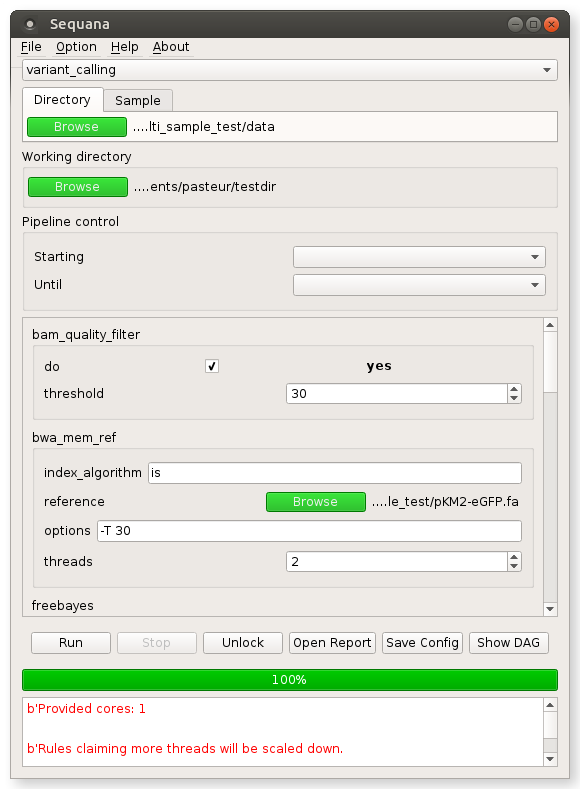
\includegraphics[scale=0.25]{../../images/sequana_finish}}

        \end{column}
        \begin{column}{0.5\textwidth}
            \only<1>{
                \begin{itemize}
                    \item Interface developed with PyQT5 and python
                    \item Wrap our snakemake pipelines to ease the usage
                    \item Usable on our cluster, which allows X11
                \end{itemize}
            }
            \only<2-6>{
            \begin{enumerate}
                \item<2-6> Choose a pipeline
                \item<3-6> Set input and output
                \item<4-6> Fill the config formular
                \item<5-6> Run the pipeline
                \item<6> Finished !
            \end{enumerate}
            }
        \end{column}
    \end{columns}
\end{frame}



\begin{frame}
\frametitle{Reference} 
 
\textbf{Sequanix: A Dynamic Graphical Interface for Snakemake Workflows} 

\vspace{.5cm}

\textit{Dimitri Desvillechabrol, Rachel Legendre, Claire Rioualen, Christiane 
Bouchier, Jacques van Helden, Sean Kennedy, Thomas Cokelaer}

\vspace{.5cm}
 
https://www.biorxiv.org/content/early/2017/07/12/162701
 
\end{frame}


 
\section{Sequana coverage}


\begin{frame}
\frametitle{Genome coverage}

\textbf{Definition:} The number of reads mapped to a specific position, $b$, 
within the reference genome. \\
\vspace{1em}
\textbf{Notation:} $ C(b)$ also denoted $C_b$\\
\vspace{1em}
\textbf{Theoretical distribution:} Poisson distribution but in practice over 
dispersed. The poisson parameter is distributed according to a Gamma hence 
leading to a negative binomial (See e.g., Linder et al 2013).
\end{frame}


\begin{frame}
\frametitle{\small Bacteria case (low/high $\mu$ components and del. region)}
\begin{center}
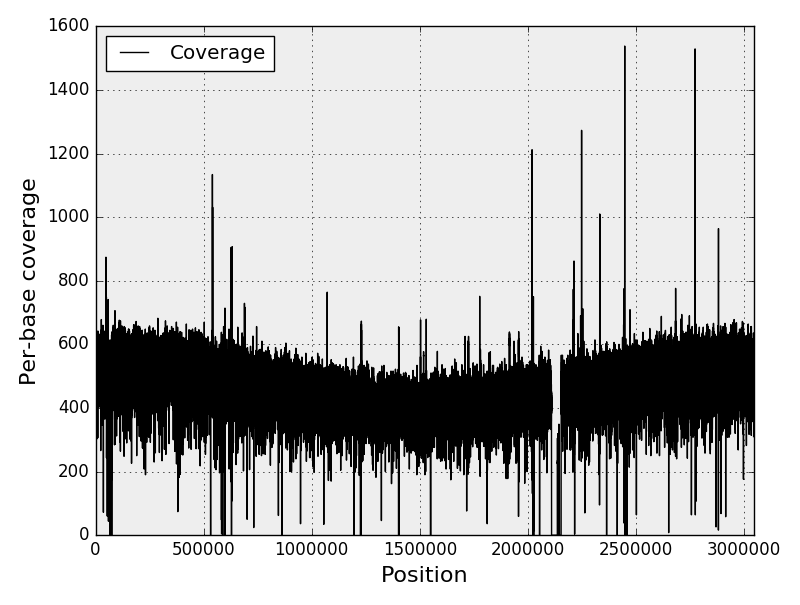
\includegraphics[height=0.9\textheight, 
width=1\textwidth]{images/coverage_bacteria.png}
%Problems (see next figures)
%   Low and high frequency trends prevent fitting of any distribution
%    Some regions are deleted.
%    Others are repeated or over covered by several folds
\end{center}
\end{frame}



\begin{frame}
\frametitle{\small Virus case}
\begin{center}
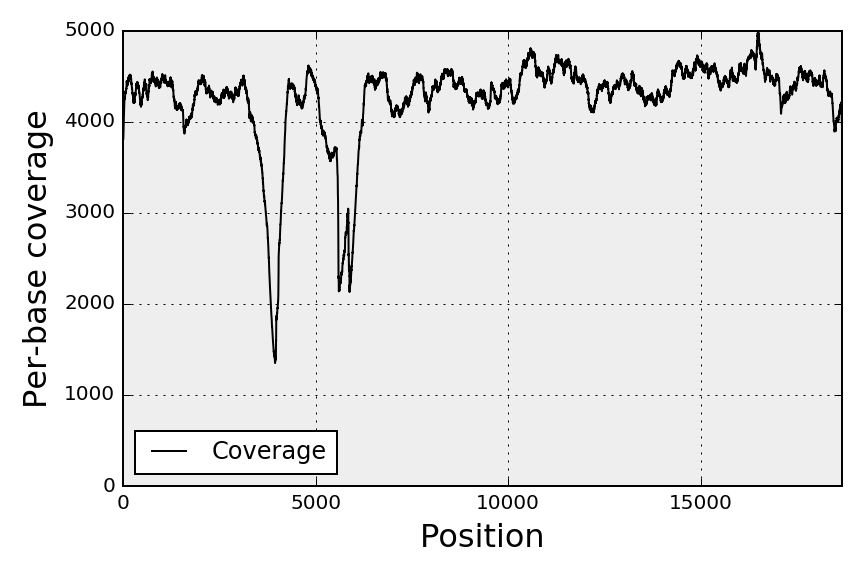
\includegraphics[height=0.9\textheight, 
width=1\textwidth]{images/coverage_virus.png}
%Problems (see next figures)
%   Low and high frequency trends prevent fitting of any distribution
%    Some regions are deleted.
%    Others are repeated or over covered by several folds
\end{center}
\end{frame}


\begin{frame}
\LARGE
\begin{block}{Question: how to automatically detect and characterise under and 
over covered genomic regions}
\end{block}

\end{frame}


\begin{frame}[fragile]
 \begin{verbatim}
1. The algorithm
   1. Detrending (running median)
   2. Mixture model estimation (Gaussian approximation)
   3. Set a statistics (z-score)
   4. Clustering (double threshold)

\end{verbatim}
\end{frame}


%%%%%%%%%%%%%%%%%%%%%%%%%%%%%%%%%%%%%%%%%%%%%%%%%%%%%%%%%%%%%%%%%%%%%%%%%%
\begin{frame}
\frametitle{1. Detrending (Normalised coverage)}
\begin{center}
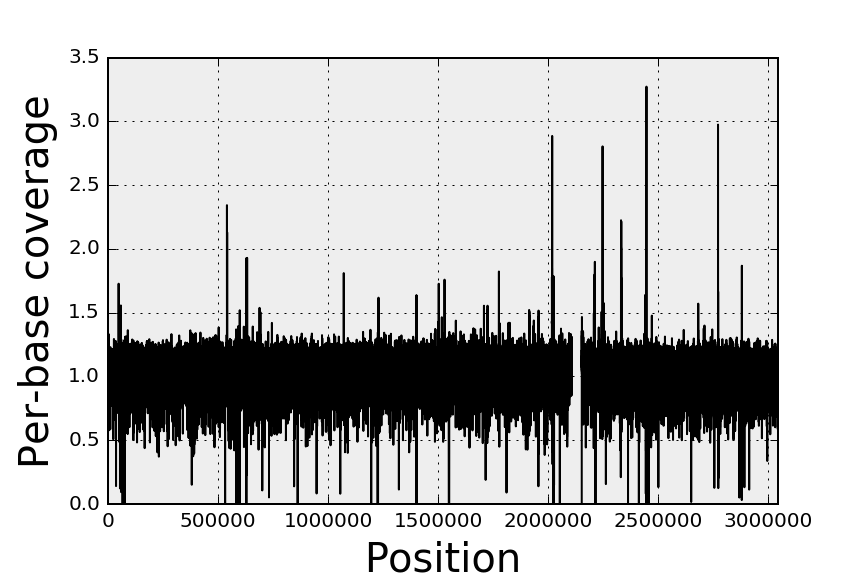
\includegraphics[height=0.8\textheight, 
    width=1\textwidth]{images/coverage_normalised.png}
\end{center} 
\end{frame}


\begin{frame}
 \frametitle{2. Building a statistics}
 
\textbf{Hypothesis 2:} The normalised genome coverage follows a 
Gaussian distribution in particular the central distribution

\begin{center}
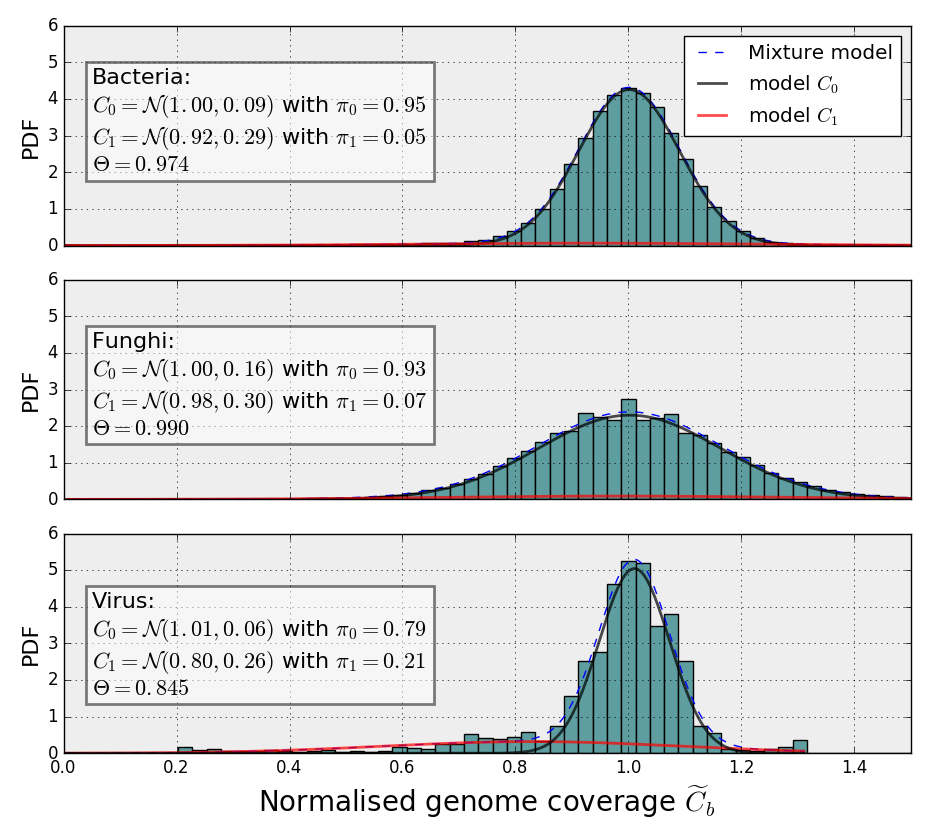
\includegraphics[height=0.7\textheight, 
    width=1\textwidth]{images/figure_em.png}
\end{center} 
\end{frame}




%%%%%%%%%%%%%%%%%%%%%%%%%%%%%%%%%%%%%%%%%%%%%%
\begin{frame}
\frametitle{C. From a constant to adaptative $z$-score}
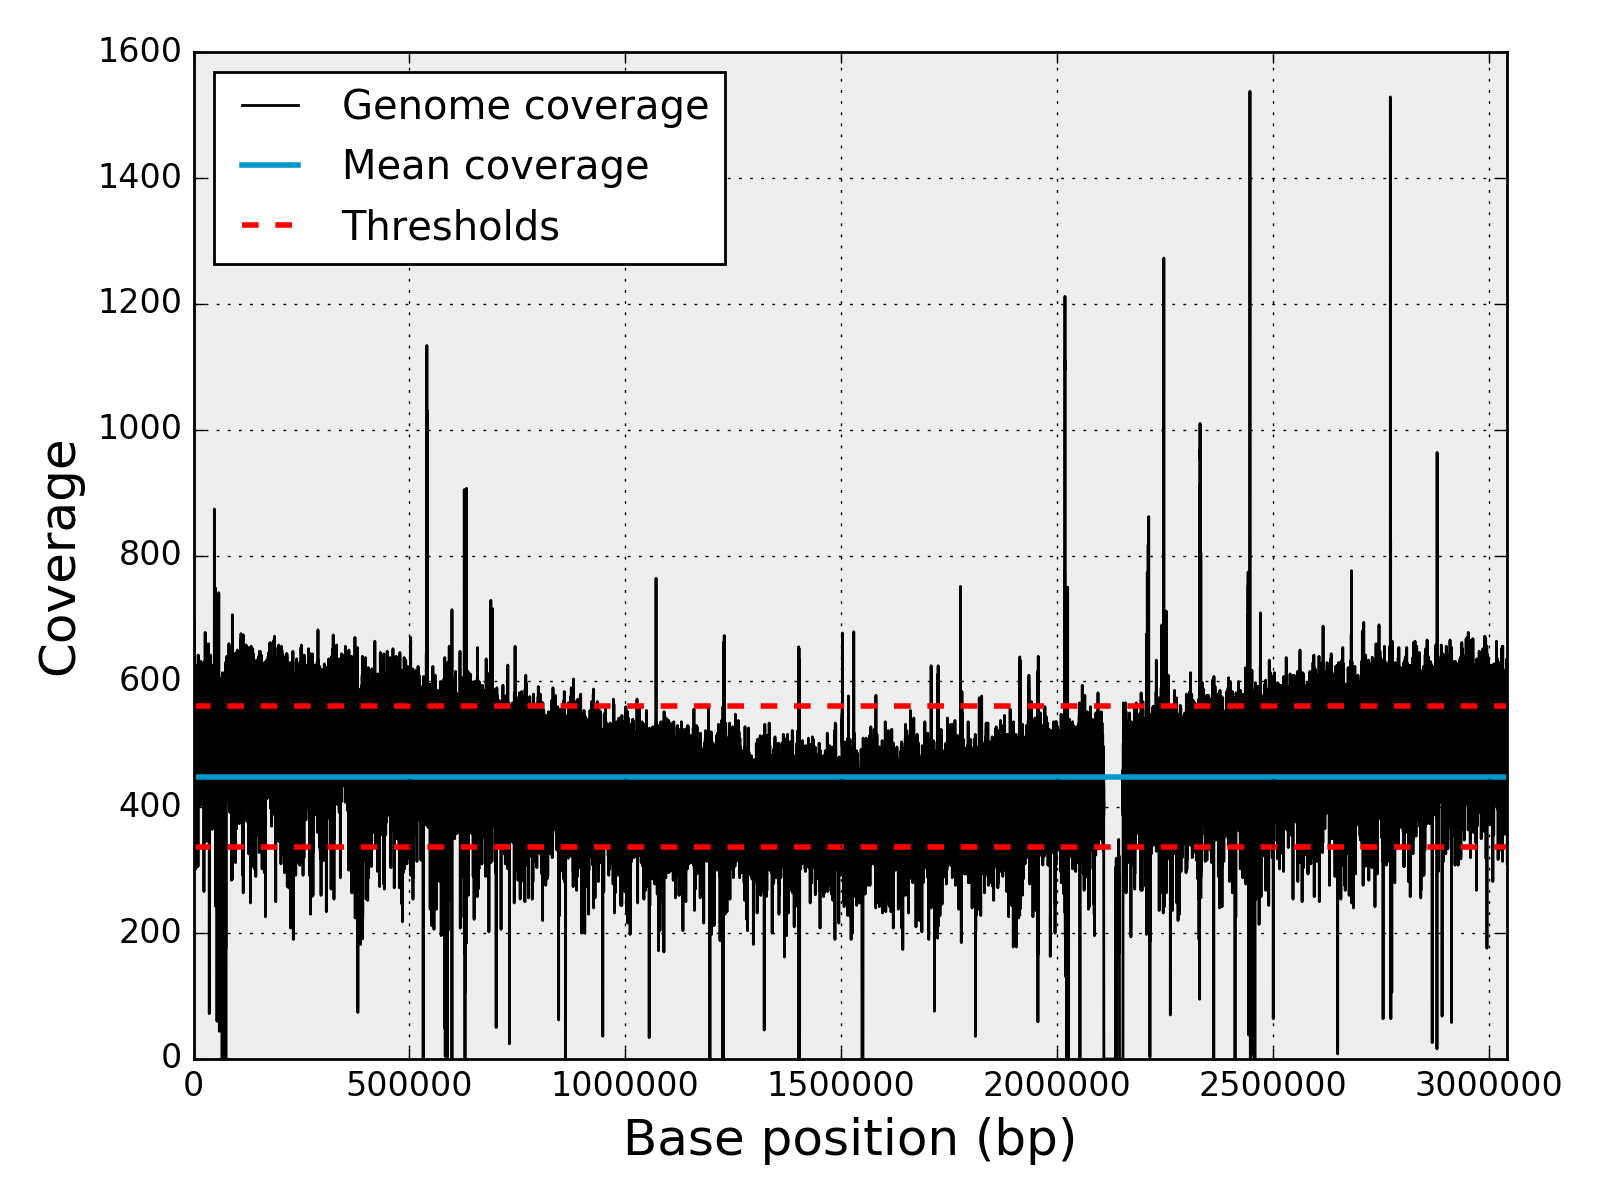
\includegraphics[height=0.9\textheight, width=1\textwidth]{images/fig1.png}
 \end{frame}
\begin{frame}
\frametitle{C. From a constant to adaptative $z$-score}
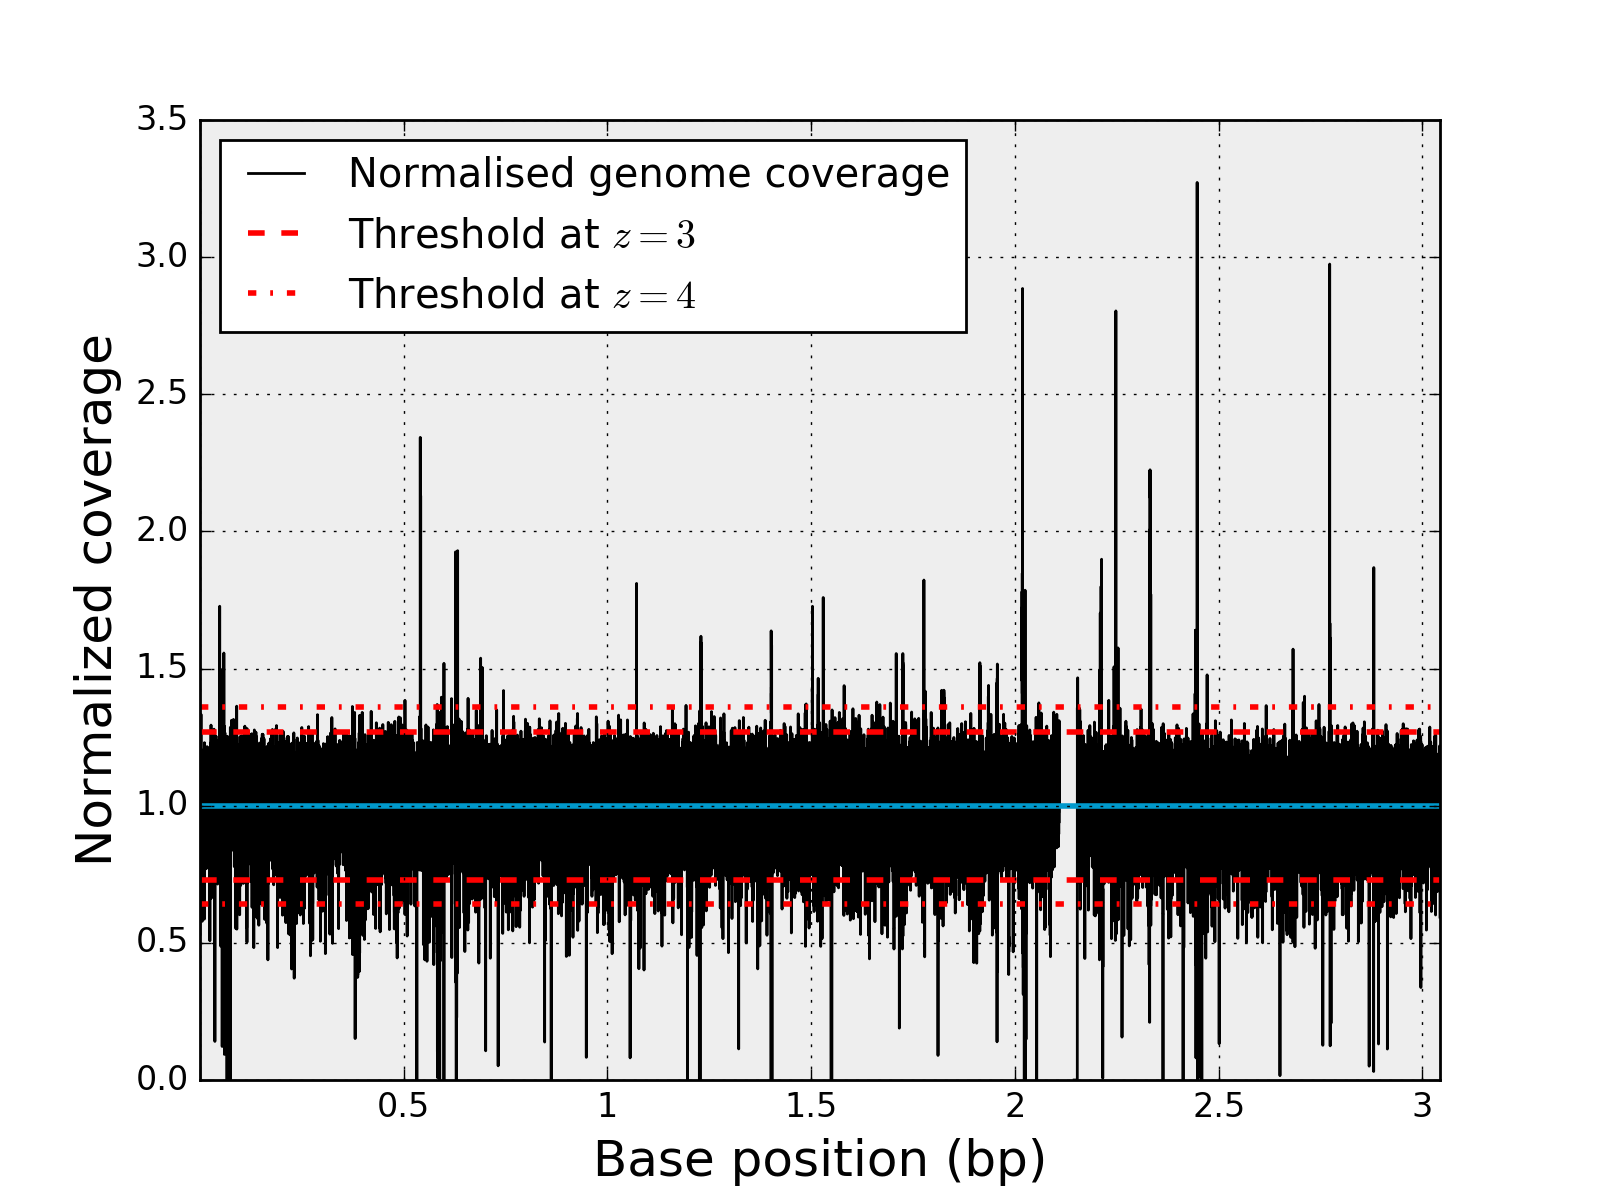
\includegraphics[height=0.9\textheight, width=1\textwidth]{images/fig2.png}
 \end{frame}
\begin{frame}
\frametitle{C. From a constant to adaptative $z$-score}
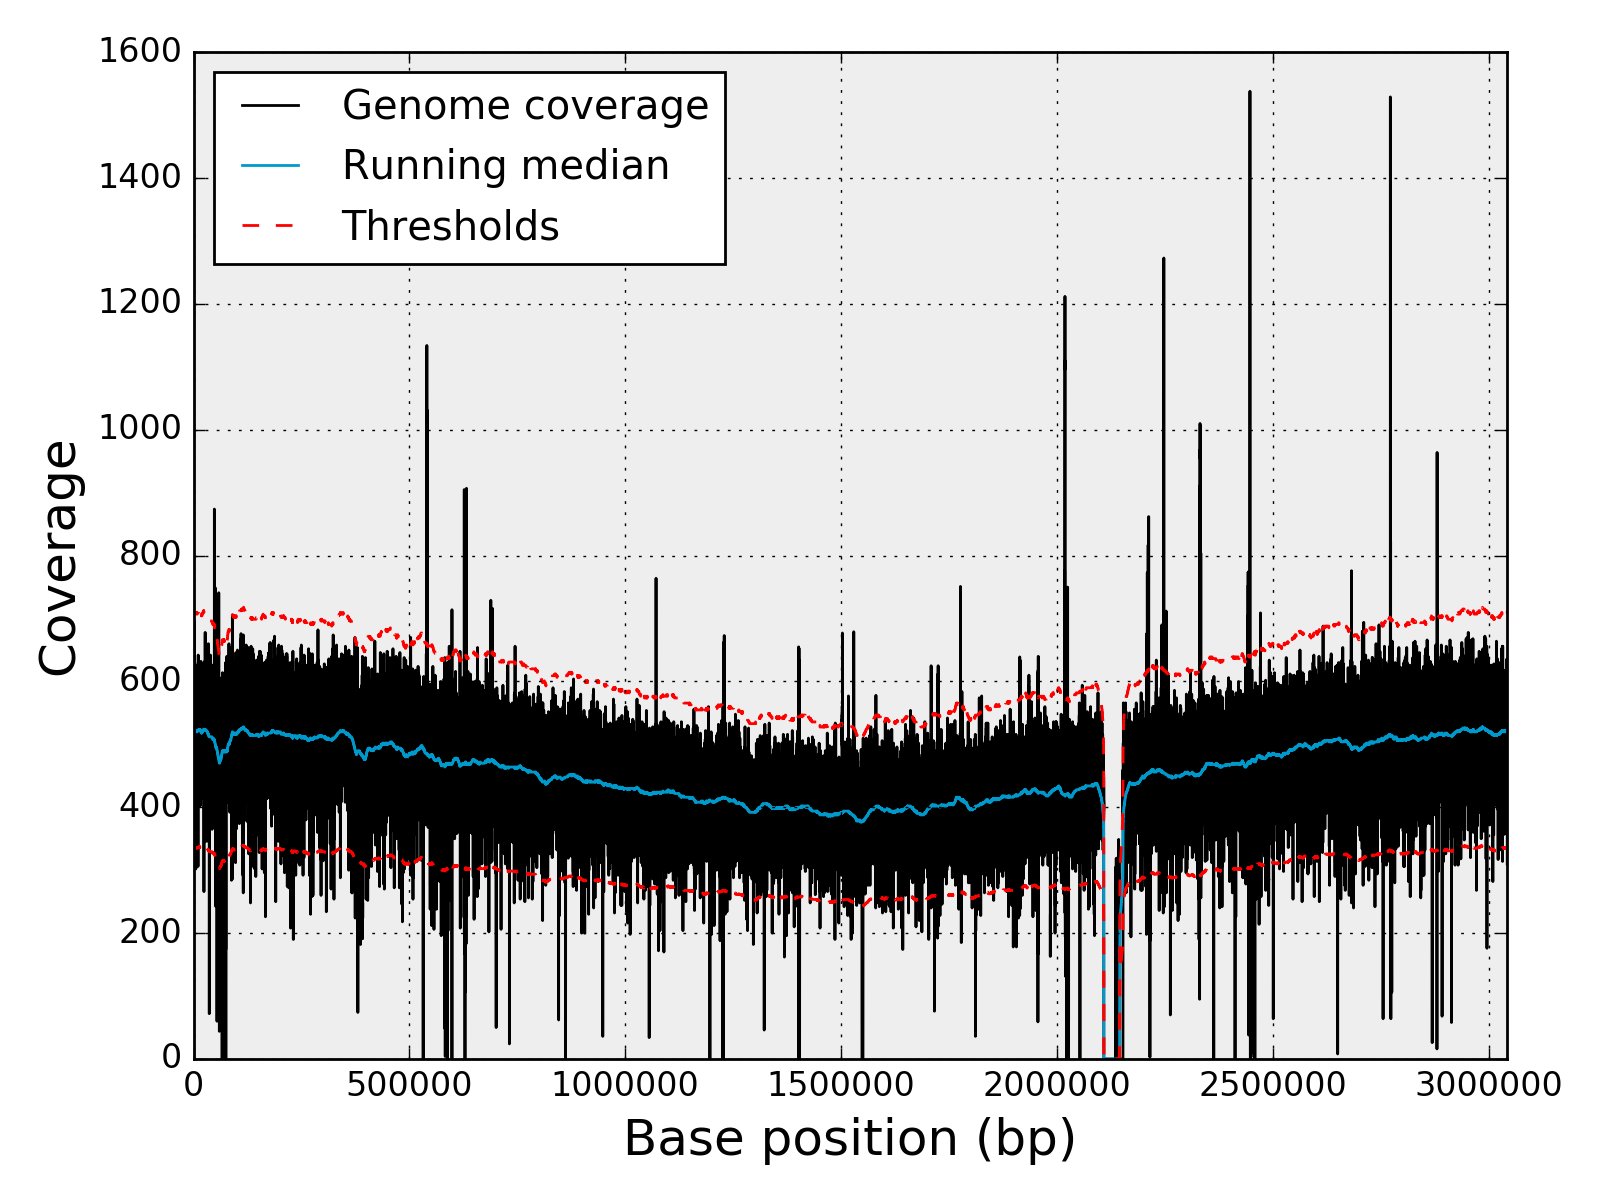
\includegraphics[height=0.9\textheight, width=1\textwidth]{images/fig3.png}
 \end{frame}



 \begin{frame}
\textbf{Detection and characterization of low and high genome coverage 
regions using an efficient running median and a double threshold approach.}
\\
\vspace{.4cm}
\textit{Dimitri Desvillechabrol, Christiane Bouchier, Sean Kennedy, Thomas
Cokelaer}
\\
\vspace{.4cm}
bioRxiv 092478; doi: http://dx.doi.org/10.1101/092478
\end{frame}


 

\section{Sequana: Continuous integration}
\input{../../slides/slide_sequana_ci_2017_oct}

\section{Summary}

\begin{frame}
 \frametitle{Summary}
Sequana is a versatile tool that provides

\begin{enumerate}
 \item A Python library dedicated to NGS analysis (e.g., tools to visualise 
standard NGS formats).
\item A set of snakemake workflows and rules dedicated to NGS 
 \item A GUI to execute them easily with Sequanix
 \item HTML reports
 \item Standalone applications:
 \begin{itemize}
    \item \textbf{sequana\_coverage} ease the extraction of genomic regions of interest and genome coverage information
    \item \textbf{sequana\_taxonomy} get a quick overview of read contents
    \item \dots
 \end{itemize}
\end{enumerate}
\end{frame}



\begin{frame}
\frametitle{You like it ? Please, add a star on our github}
    https://github.com/sequana/sequana/stargazers
    \centering
    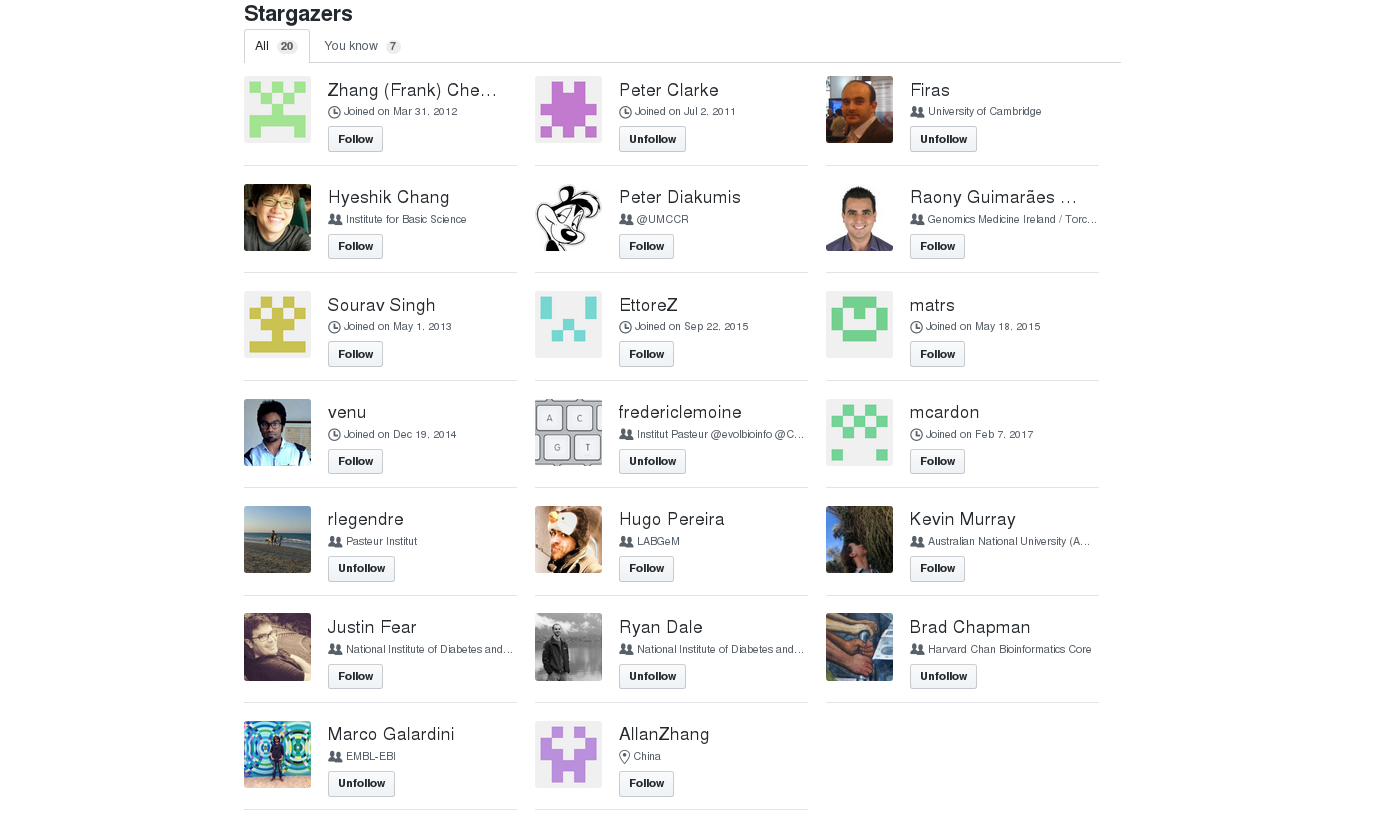
\includegraphics[scale=0.28]{images/stargazers.png}\\
\end{frame}


\begin{frame}
\frametitle{You like it ? }
\centering
Join us ! add rules and pipelines !
\end{frame}



    
    



\begin{frame}
 \frametitle{Acknowledgements}

 \begin{itemize}
  \item Dimitri Desvillechabrol (variant calling, denovo, sequana, sequanix)
  \item Rachel Legendre (Transcriptomics)
  \item M\'elissa Cardon (pacbio)
  \item Biomics users (Institut Pasteur)
 \end{itemize}
 
\end{frame}


\begin{frame}
\centering
\vspace{2cm}
\LARGE
 Thank you 
 
 \vspace{2cm}
 
 \small
 Slides available on http://github.com/sequana/sequana\_presentations/
\end{frame}




\end{document}
